\documentclass{article}
\usepackage{polyglossia}
\usepackage[a4paper, total={6in, 8in}]{geometry}
\usepackage{graphicx}
\usepackage{listings}
\usepackage{color}
\usepackage{pdfpages}
\usepackage{hyperref}
\usepackage{pdflscape}
\usepackage{float}
\graphicspath{ {./images/} }
\setmainlanguage{ukrainian} 
\setotherlanguage{english}
\setmainfont{CMU Serif}
\setsansfont{CMU Sans Serif}            
\setmonofont{CMU Typewriter Text}
\definecolor{mygreen}{rgb}{0,0.6,0}
\definecolor{mygray}{rgb}{0.5,0.5,0.5}
\definecolor{mymauve}{rgb}{0.58,0,0.82}

\lstset{ 
backgroundcolor=\color{white},   % choose the background color; you must add \usepackage{color} or \usepackage{xcolor}; should come as last argument
basicstyle=\ttfamily,            % the size of the fonts that are used for the code
breakatwhitespace=false,         % sets if automatic breaks should only happen at whitespace
breaklines=true,                 % sets automatic line breaking
commentstyle=\color{mygreen},    % comment style
frame=single,	                   % adds a frame around the code
keywordstyle=\color{blue},       % keyword style
language=Java,                   % the language of the code
numbers=left,                    % where to put the line-numbers; possible values are (none, left, right)
stringstyle=\color{mymauve},     % string literal style
tabsize=2,	                   % sets default tabsize to 2 spaces
title=\lstnam,                   % show the filename of files included with \lstinputlisting; also try caption instead of title
showspaces=false
}
\begin{document}
\begin{titlepage}
	\begin{center} \large
		Національний університет "Києво-Могилянська Академія"\\Факультет інформатики
	\end{center}
	\vspace*{\fill}
	\begin{center}
		
\includegraphics[width=0.5 \textwidth]{kma}
	\end{center}
	\vspace*{\fill}
	\begin{center} \LARGE
		Freshmaze
	\end{center}
	\vspace*{\fill}
	\leftskip=0.5\textwidth
	Виконала Команда "DAR": Омельчук Руслан, Сукайло Дмитро, Трохимчук Артем Студенти І курсу НаУКМА Факультет Інформатики
	Спеціальність: інженерія програмного забезпечення, гр.3
	\\Викладач: Кирієнко Оксана Валентинівна
	% \maketitle
	\vspace*{\fill}
	\begin{center}
		Київ --- 2023
	\end{center}
\end{titlepage}
\section{Постановка і аналіз задачі}
Розробити гру, в процесі використовувати Git для розподіленої розробки
програмного забезпечення. Реалізувати програму інтерактивної графічної
гри, графічного інтерфейсу користувача.
\subsection{Опис ігрового процесу}
\textbf{Freshmaze} - це гра в жанрі roguelike, суть якої полягає у проходженні гравцем процедурно
згенерованих рівнів підземелля, на якому він зустрічає ворогів та нагороди.
У одній із кімнат розміщується перехід на наступний рівень, де збільшується складність.
Гра може тривати або нескінченно (до смерті гравця) або мати обмежену кількість рівнів
(це залежить від подальшої реалізації).
Після смерті гравця ігровий процес починається спочатку.

\subsection{Аналіз задачі}
Особливістю створення ігор є динамічність розробки та широкий простір для змін,
оскільки у процесі розробки може виявитися, що певні, коректно реалізовані, з погляду коду,
механіки не є "цікавими" для гри або потребують значних змін.
Тому на початковому етапі можна виділити лише основні підзадачі:

\begin{enumerate}
	\item Процедурна генерація рівнів
	\item Гравець та його переміщення
	\item Система бою та штучний інтелект ворогів
	\item Система нагород та бонусів
\end{enumerate}

Не варто також забувати про створення графічних ресурсів та
цілісного ігрового дизайну.

\section{Розподіл ролей в середині команди}
Згідно з названими вище причинами, тобто оскільки кожен аспект гри може зайняти
непрогнозовану кількість часу, наша команда вирішила застосувати
динамічний підхід у розподілі ролей. Проте є початкові напрямки роботи які
обрали члени команди:
\begin{itemize}
	\item Руслан був тімлідом, зайнявся генерацією ідей, та основними розробками гри;
	\item Артем --- створив гравця та системи бою, налагодження переходу між рівнями;
	\item Дмитро --- створив систему нагород, відеорекламу та звіт.
\end{itemize}
\section{Cтруктура програми}
\section{Структура програми}
\begin{figure}[H]
	\centering
	\includegraphics[width=0.9 \textwidth]{uml.pdf}
	\caption{Діаграма класів}
\end{figure}
\section{Опис методів та класів}
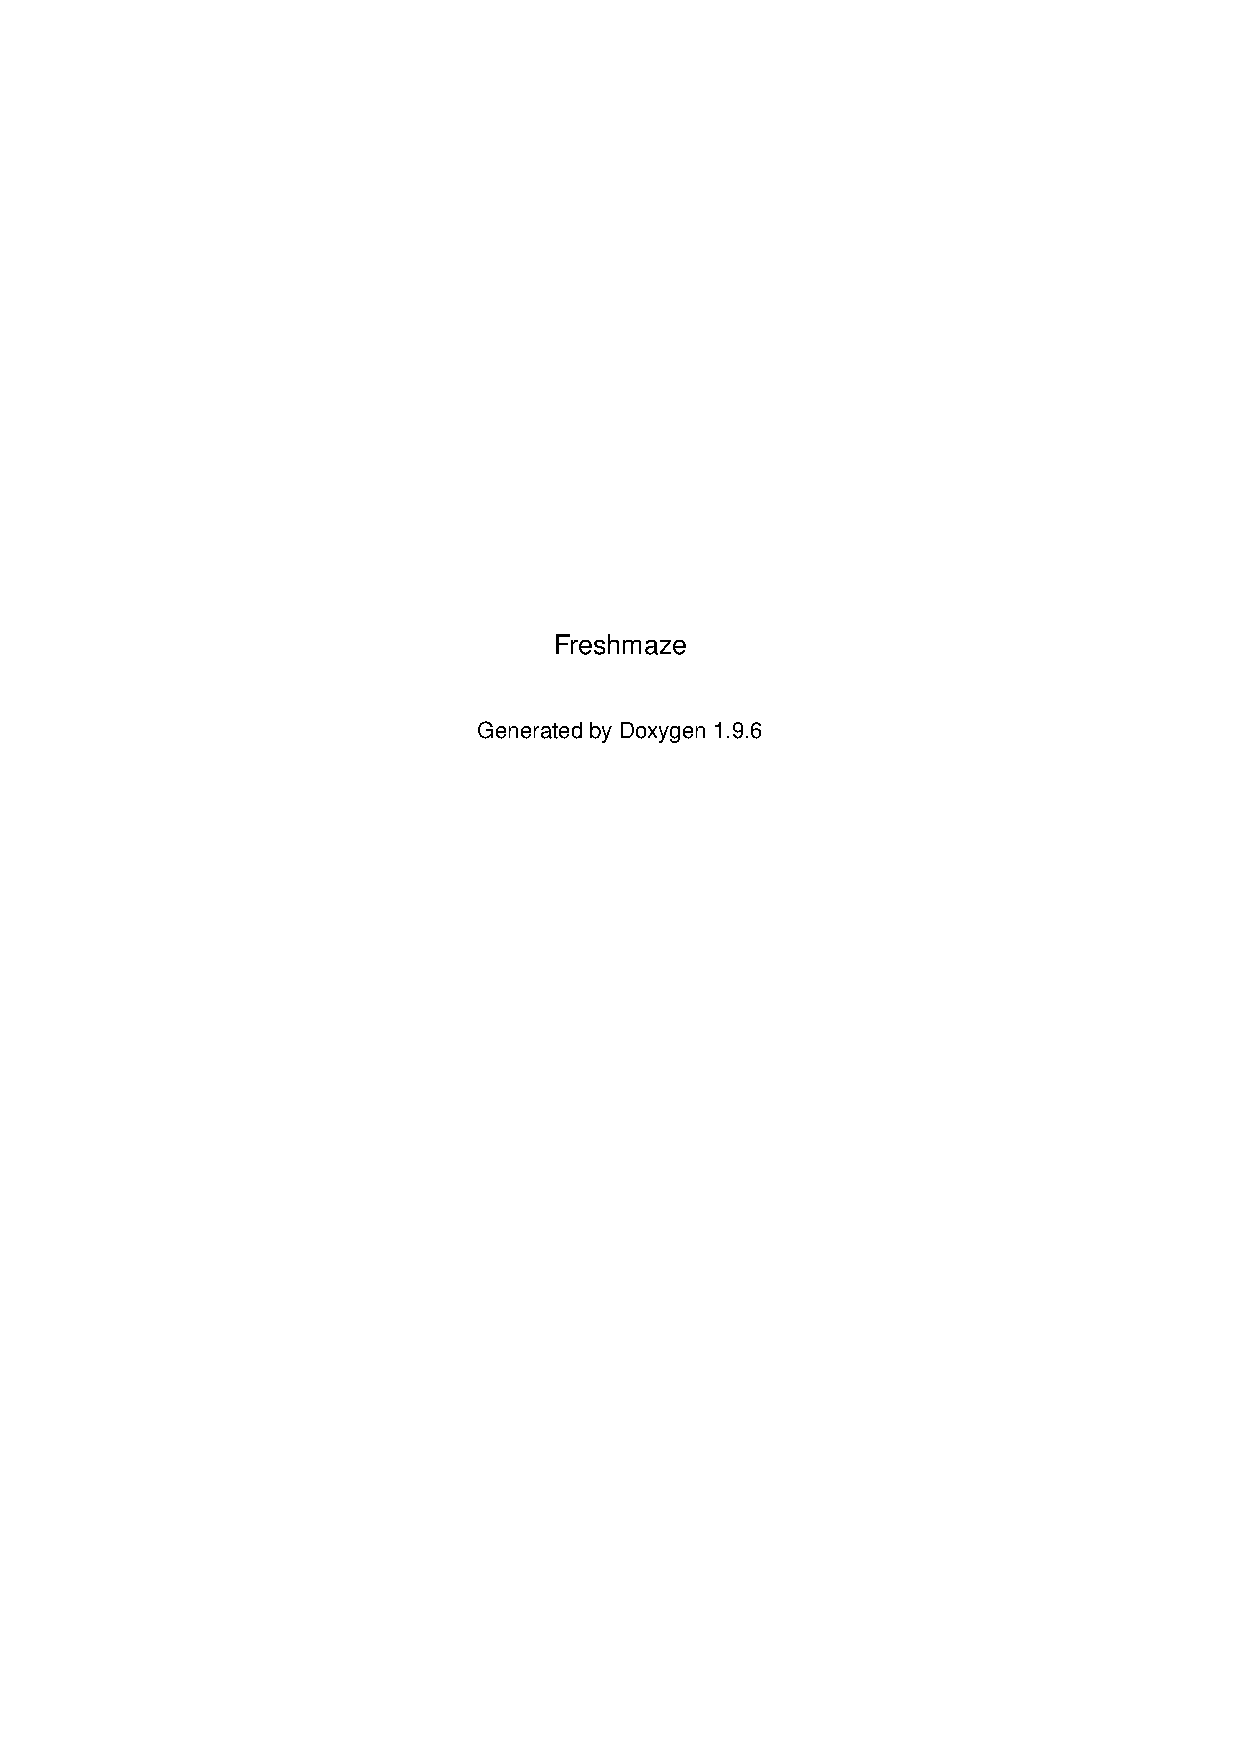
\includepdf[pages=-]{../docs/latex/refman.pdf}
\section{Інструкція користувача}
При запуску програми користувач бачить початкове вікно реалізованої
програми:
\begin{figure}[H]
	\centering
	\includegraphics[width=0.9 \textwidth]{1}
	\caption{Головний екран}
\end{figure}
Гравець має натиснути пробіл, щоб розпочати гру. Далі він побачить свою
початкову позицію. Наприклад:
\begin{figure}[H]
	\centering
	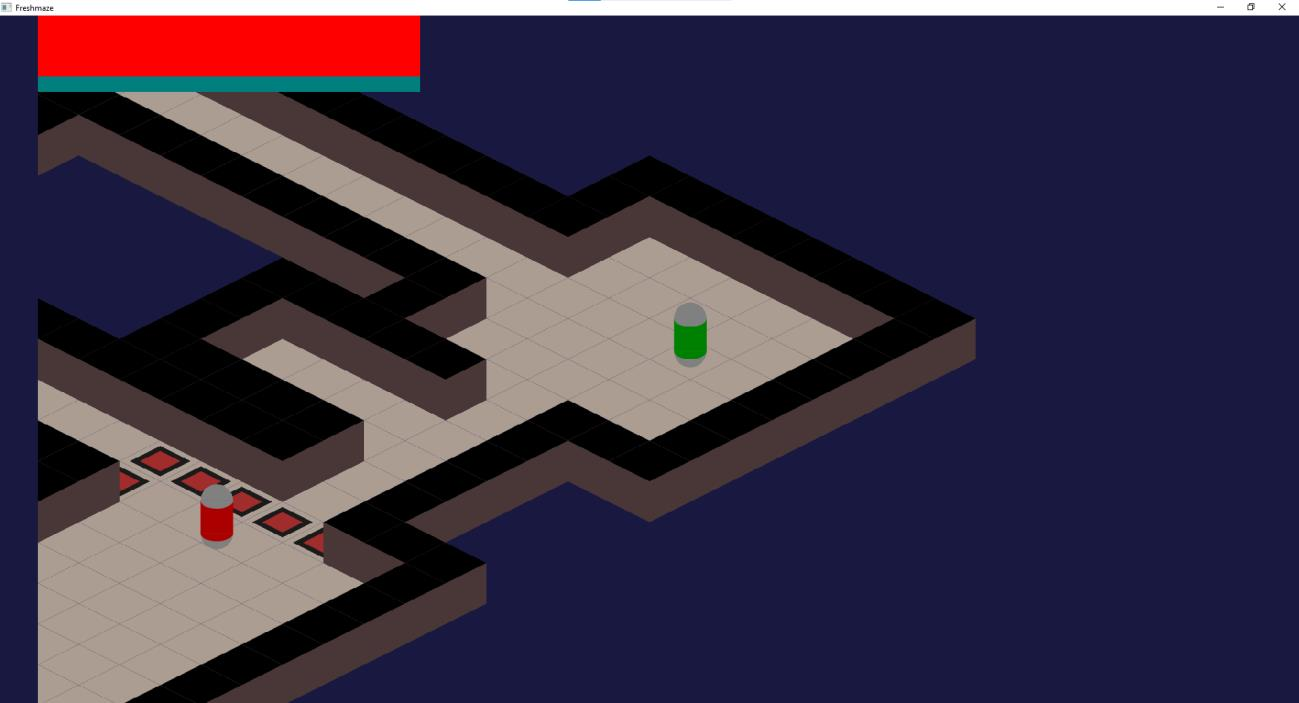
\includegraphics[width=0.9 \textwidth]{2}
	\caption{Початок гри}
\end{figure}
Користувач може рухатися за допомогою таких клавіш:
\begin{figure}[H]
	\centering
	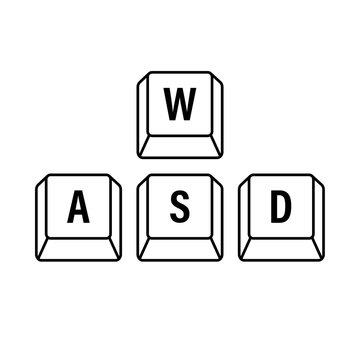
\includegraphics[width=0.5 \textwidth]{3}
	\caption{Клавіші WASD}
\end{figure}
\begin{itemize}
	\item W – рухатися вперед
	\item A – рухатися ліворуч
	\item S – рухатися назад
	\item D – рухатися праворуч
\end{itemize}
Також гравець може включити вільну камеру, щоб проглянути, на якій карті
він знаходиться та знайти кімнату де портал. Щоб включити камеру треба
натиснути на англійську клавішу P. Пересувати камеру можна за допомогою
клавіш I,J,K,L. Ці клавіші є відповідними для таких: W,A,S,D:
\begin{figure}[H]
	\centering
	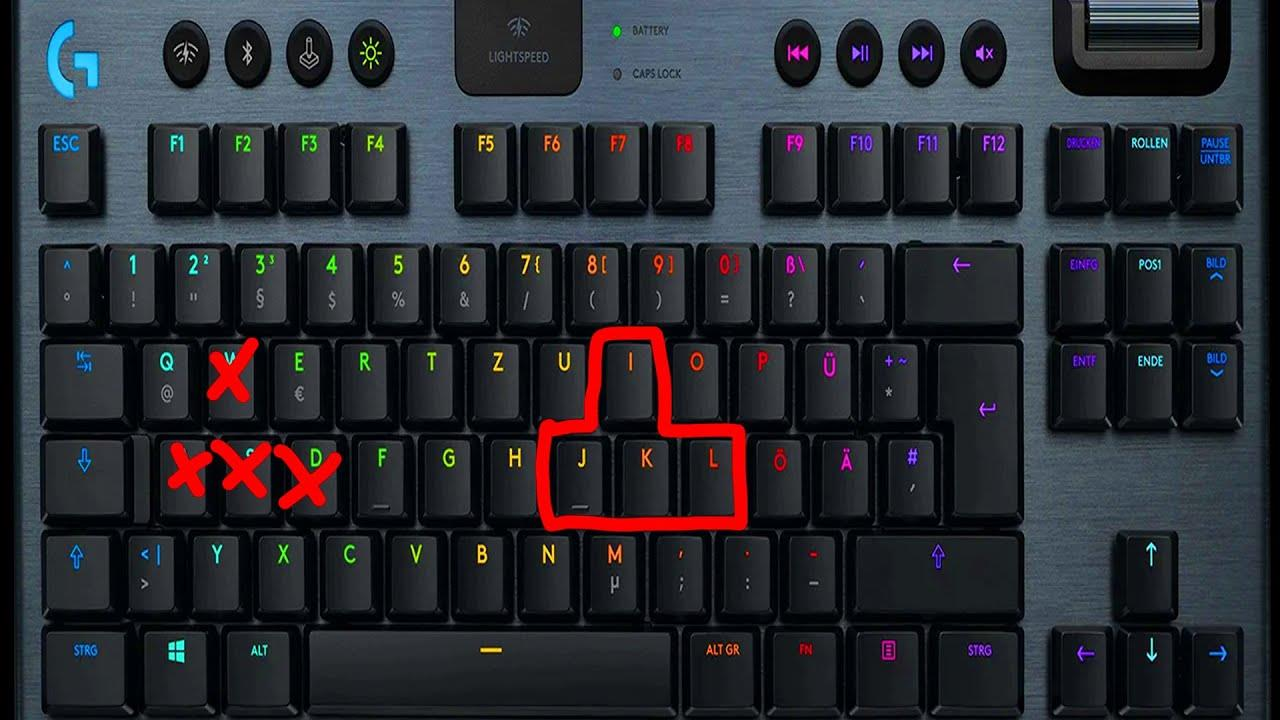
\includegraphics[width=0.9 \textwidth]{4}
	\caption{Клавіші для управління грою}
\end{figure}
\section{Проблеми, що виникали}
\begin{enumerate}
	\item Проблема з підтягуванням бібліотек та реалізації. Вирішення: вирішив все робити на Свінгу.
	\item Проблема з великим вмістом інформації в екселі, при побудові та аналізі графіка функції. Вирішення: зменшив крок параметра функції.
	\item Проблема відображення графіка. Вирішення: прочитання декількох онлайн ресурсів, що допомогло поправити код.
\end{enumerate}
\section{Висновки}
\textbf{Висновок:} покращення навичок написання коду на Свінгу. А також
здобуті навички пошуку інформації для способів вирішення
різноманітних проблем.
\section*{Програмний код}

\lstinputlisting[title=FreshmazeGame.java]{../core/src/com/dar/freshmaze/FreshmazeGame.java}
\lstinputlisting[title=GameScreen.java]{../core/src/com/dar/freshmaze/screens/GameScreen.java}
\lstinputlisting[title=Graph.java]{../core/src/com/dar/freshmaze/common/Graph.java}
\lstinputlisting[title=LevelBitmap.java]{../core/src/com/dar/freshmaze/level/bitmap/LevelBitmap.java}
\lstinputlisting[title=LevelGraph.java]{../core/src/com/dar/freshmaze/level/graph/LevelGraph.java}
\lstinputlisting[title=LevelNode.java]{../core/src/com/dar/freshmaze/level/graph/LevelNode.java}
\lstinputlisting[title=LevelNodeGenerationRules.java]{../core/src/com/dar/freshmaze/level/graph/LevelNodeGenerationRules.java}
\lstinputlisting[title=LevelNodeGenerator.java]{../core/src/com/dar/freshmaze/level/graph/LevelNodeGenerator.java}
\lstinputlisting[title=LevelTilemap.java]{../core/src/com/dar/freshmaze/level/tilemap/LevelTilemap.java}
\lstinputlisting[title=ChestTile.java]{../core/src/com/dar/freshmaze/level/tilemap/tiles/ChestTile.java}
\lstinputlisting[title=DynamicTile.java]{../core/src/com/dar/freshmaze/level/tilemap/tiles/DynamicTile.java}
\lstinputlisting[title=DynamicInteractableTile.java]{../core/src/com/dar/freshmaze/level/tilemap/tiles/DynamicInteractableTile.java}
\lstinputlisting[title=EntranceTile.java]{../core/src/com/dar/freshmaze/level/tilemap/tiles/EntranceTile.java}
\lstinputlisting[title=SpikesTile.java]{../core/src/com/dar/freshmaze/level/tilemap/tiles/SpikesTile.java}
\lstinputlisting[title=TeleportTile.java]{../core/src/com/dar/freshmaze/level/tilemap/tiles/TeleportTile.java}
\lstinputlisting[title=BattleLevelRoom.java]{../core/src/com/dar/freshmaze/level/tilemap/rooms/BattleLevelRoom.java}
\lstinputlisting[title=FinalLevelRoom.java]{../core/src/com/dar/freshmaze/level/tilemap/rooms/FinalLevelRoom.java}
\lstinputlisting[title=LevelRoom.java]{../core/src/com/dar/freshmaze/level/tilemap/rooms/LevelRoom.java}
\lstinputlisting[title=SpawnLevelRoom.java]{../core/src/com/dar/freshmaze/level/tilemap/rooms/SpawnLevelRoom.java}
\lstinputlisting[title=SortedIsometricTiledMapRenderer.java]{../core/src/com/dar/freshmaze/level/tilemap/SortedIsometricTiledMapRenderer.java}
\lstinputlisting[title=SpikeGenerator.java]{../core/src/com/dar/freshmaze/level/tilemap/SpikeGenerator.java}
\lstinputlisting[title=Dungeon.java]{../core/src/com/dar/freshmaze/level/Dungeon.java}
\lstinputlisting[title=EnemyGenerator.java]{../core/src/com/dar/freshmaze/level/EnemyGenerator.java}
\lstinputlisting[title=Level.java]{../core/src/com/dar/freshmaze/level/Level.java}
\lstinputlisting[title=RectangleUtil.java]{../core/src/com/dar/freshmaze/util/RectangleUtil.java}
\lstinputlisting[title=IsometricUtil.java]{../core/src/com/dar/freshmaze/util/IsometricUtil.java}
\lstinputlisting[title=TimeUtil.java]{../core/src/com/dar/freshmaze/util/TimeUtil.java}
\lstinputlisting[title=Bob.java]{../core/src/com/dar/freshmaze/entities/Bob.java}
\lstinputlisting[title=Enemy.java]{../core/src/com/dar/freshmaze/entities/Enemy.java}
\lstinputlisting[title=HealthBonus.java]{../core/src/com/dar/freshmaze/entities/HealthBonus.java}
\lstinputlisting[title=Entity.java]{../core/src/com/dar/freshmaze/entities/Entity.java}
\lstinputlisting[title=PhysActor.java]{../core/src/com/dar/freshmaze/entities/PhysActor.java}
\lstinputlisting[title=RectIndicator.java]{../core/src/com/dar/freshmaze/indicator/RectIndicator.java}
\lstinputlisting[title=WorldContactListener.java]{../core/src/com/dar/freshmaze/world/WorldContactListener.java}
\lstinputlisting[title=DepthSortedStage.java]{../core/src/com/dar/freshmaze/graphics/DepthSortedStage.java}
\lstinputlisting[title=ScreenTransition.java]{../core/src/com/dar/freshmaze/ui/ScreenTransition.java}

\listoffigures
\end{document}












